To improve the robustness of reading and achieve ultra-low BER, this paper proposes a time-based sensing scheme with a built-in read control loop to support both single readout for normal application and multiple readout for massive repeated sampling.
This section describes the circuit design and detailed analysis of the proposed time-based sensing scheme.

The proposed time-based sensing circuit is depicted in Fig. \ref{fig_prop_circuit}(a), which consists of (1) a voltage-time converter (VTC) to convert the BL voltage to a time delay, (2) a power gating inverter (PGI) to minimize the short-circuit current, (3) a charge sharing-induced error compensation (CSEC) circuit to eliminate the charge sharing-induced error and improve the read margin, (4) a built-in timing control loop for different reading modes, and (5) a DFF to compare and store the state. 

A low precharge voltage ($V_{PRE}$ = 300 mV) is applied to BL through an NMOS transistor. The sensing circuit stays in the precharge (reset) phase ($V_{BL}$ = $V_{PRE}$) when the precharge enable signal $EN\_PRE$ is asserted. When $EN\_PRE$ is deasserted and a wordline is selected, $V_{BL}$ is discharged with different speeds according to the bitcell state, resulting in the development of $V_{BL}$ for sensing. During this time, the enable signal $EN\_VTC$ is activated to enable the VTC and convert the bitline voltage $V_{BL}$ to the time delay signal. The capacitor node voltage $V_C$ is initially precharged to $V_{DD}$ when the enable signal $EN\_VTC$ is low. The signal $EN\_VTC$ is activated when the sensing phase begins, and the capacitor node voltage $V_C$ is discharged by the current $I_{DISCH}$, which is inversely proportional to $V_{BL}$. The discharge voltage $V_C$ is, thereafter, shaped by a cascaded inverter to regenerate a sharp-edge signal $V_{out}$, which reflects the bitcell state indirectly. 
Both enable signals $EN\_PRE$ and $EN\_VTC$ are generated by the sensing enable signal  $EN\_SNS$ and the timing control loop. 
Fig. \ref{fig_prop_circuit}(b) illustrates the waveforms of the critical nodes for different RRAM states in different readout modes, where the solid and dashed lines represent the RRAM in LRS and HRS, respectively.
We will analyze the design details of each block in the following subsections.


\subsection{Voltage-to-Time Converter (VTC)}
The basic principle of VTC designs is to charge (or discharge) a capacitor from its initial voltage to a certain level and subsequently detect the time when the voltage across the capacitor crosses the threshold voltage. The ramp-based VTC generates a fixed ramp using a constant current source integrated over a capacitor and compares the ramp with the input-controlled threshold voltage \cite{naraghi20109,weng2016continuous}. The current-starved-inverter (CSI) based VTC generates the current controlled by the applied input signal and compares the voltage across the capacitor with a fixed threshold voltage \cite{zhu2016skew,chen20140,macpherson20135gs}.
Among these architectures, the CSI-based VTC topology is compact and suitable for high-speed applications \cite{macpherson20135gs}.

This work employs the CSI-based VTC structure to convert the bitline voltage into a pulse delay, considering its low power consumption, high speed, and small silicon area overhead.  
As shown in Fig. \ref{fig_prop_circuit}, when the enable signal $EN\_VTC$ is low, M$_1$ resets the capacitor node $V_C$ to $V_{DD}$; when $EN\_VTC$ is high, M$_3$ starts to discharge $V_C$ with a current $I_{DISCH}$ controlled by the bitline voltage $V_{BL}$. 
When the VTC receives a rising transition in $EN\_VTC$, it discharges the capacitor node $V_C$ and exhibits a gate delay expressed as
\begin{align}
\label{eq_delay}
T_{delay} &= C\frac{V_{DD}-V_{TRIP}}{I_{DISCH}}
\end{align}
where $V_{DD}$ is the supply voltage, $V_{TRIP}$ is the trip voltage of the subsequent inverter, $C$ is the total capacitor at the node $V_C$ (including MOS capacitance and parasitic capacitance), and $I_{DISCH}$ is the current delivered by the pull-down network of the CSI. $I_{DISCH}$ is essentially equal to the current delivered by $M_3$, reflecting the bitline voltage $V_{BL}$. 

\begin{figure}[!t]
\centerline
{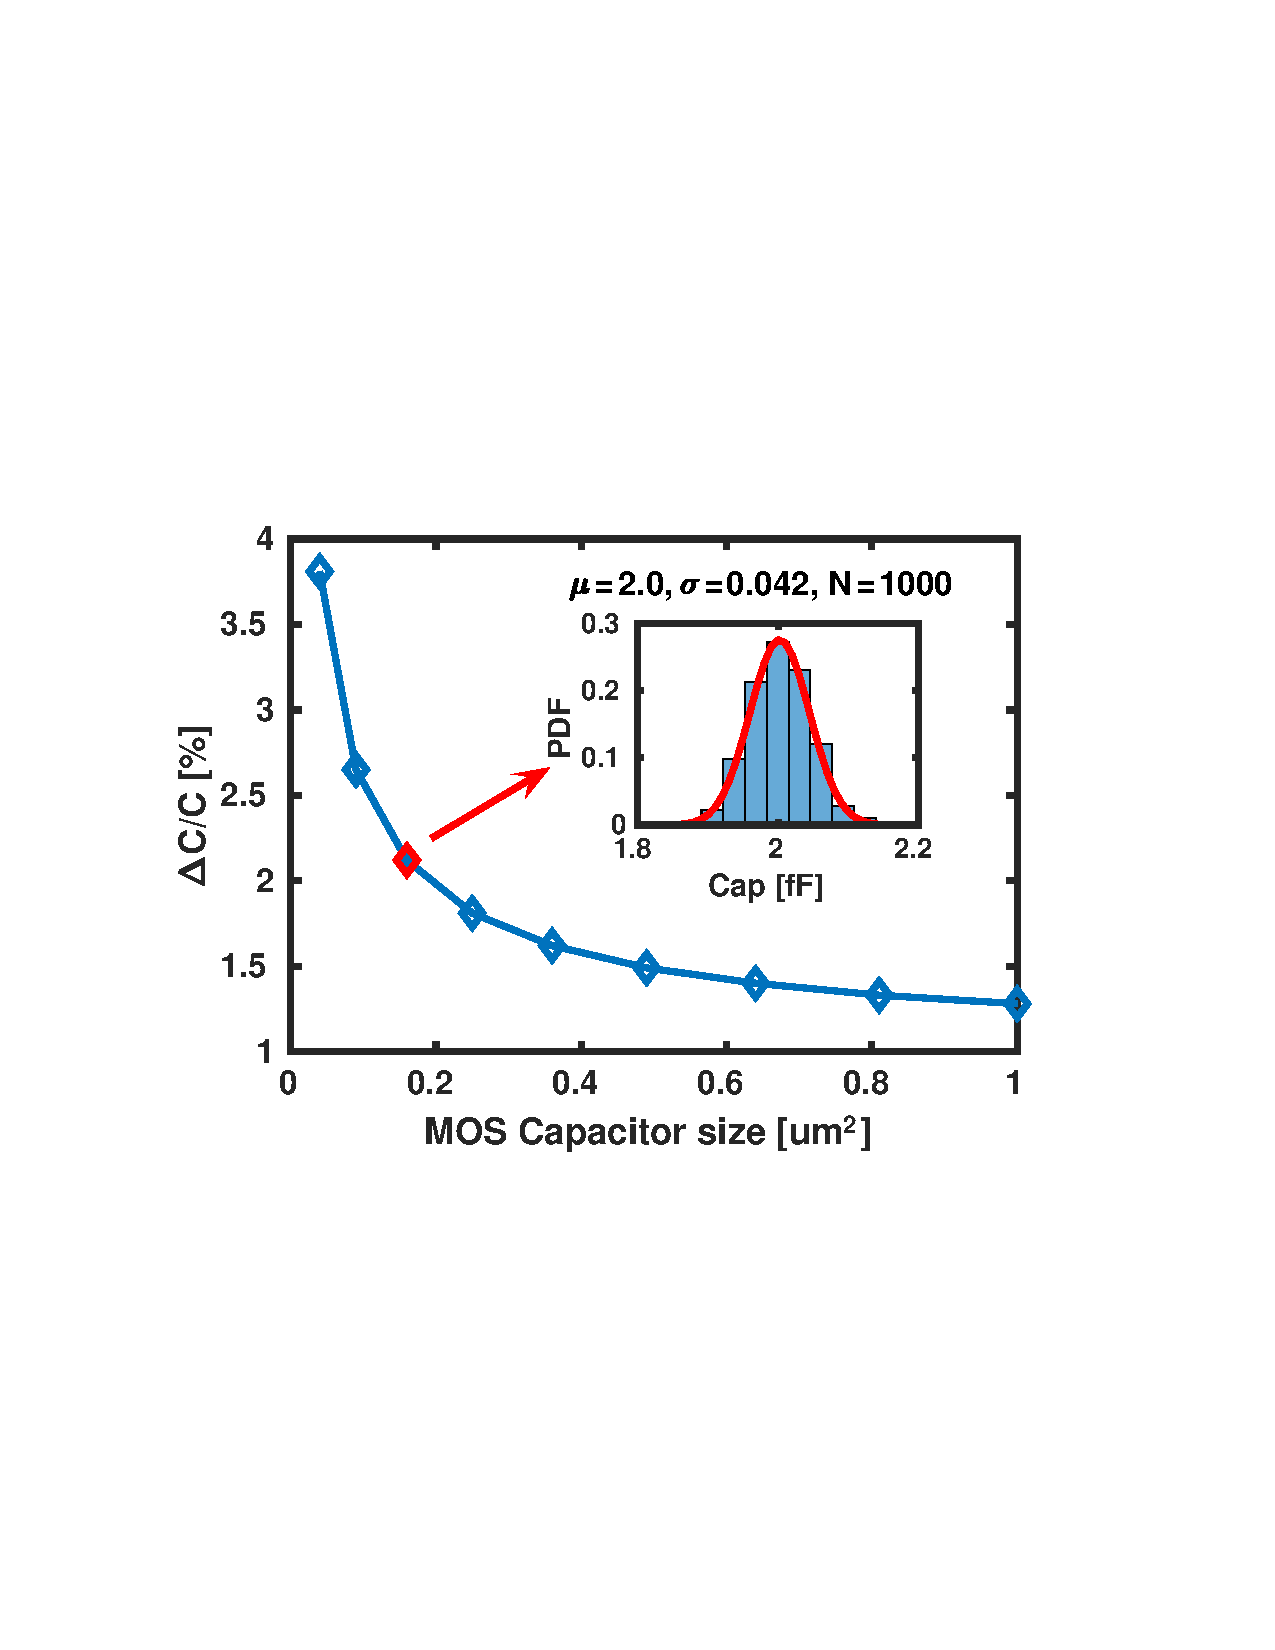
\includegraphics[width=0.46\textwidth]{fig/moscap.pdf}}
\caption{MOS capacitor mismatch for different capacitor sizes and the capacitor distribution when the MOS size is $W \times L=0.16~\rm \micro m^2$.}
\label{fig_moscap}
\end{figure}

One important trade-off in the area comes from the MOS capacitor -- a large capacitor minimizes the discharge time variations caused by mismatch at the cost of area overhead. Monte Carlo (MC) simulations with device mismatches and process variations are presented in Fig. \ref{fig_moscap}. In our design, the MOS capacitor size is selected as $W \times L=0.16~\rm \micro m^2$, resulting in a mean capacitance value of $2~\rm fF$ and a standard deviation of $42~\rm aF$. The normalized variance of capacitor is $\Delta C/C = 2.1\%$.
% \textcolor{blue}{Compared with other parts, the capacitor variation is small, }
SPICE simulations show that it is a good balance between performance and area. 

Since $V_{BL}$ is limited to the precharge voltage ($V_{PRE}$=300 mV), it is necessary to increase the size of the pull-down transistor M$_3$ to distinguish the current in different states and attenuate the effect of mismatch. As a result, the parasitic capacitance at the drain of M$_3$ is not negligible, leading to charge sharing-induced error at the transition of $EN\_VTC$. We will explain and address this issue in detail next.

\subsection{Charge Sharing-induced Error Compensation (CSEC)}

\begin{figure}[!t]
\centerline
{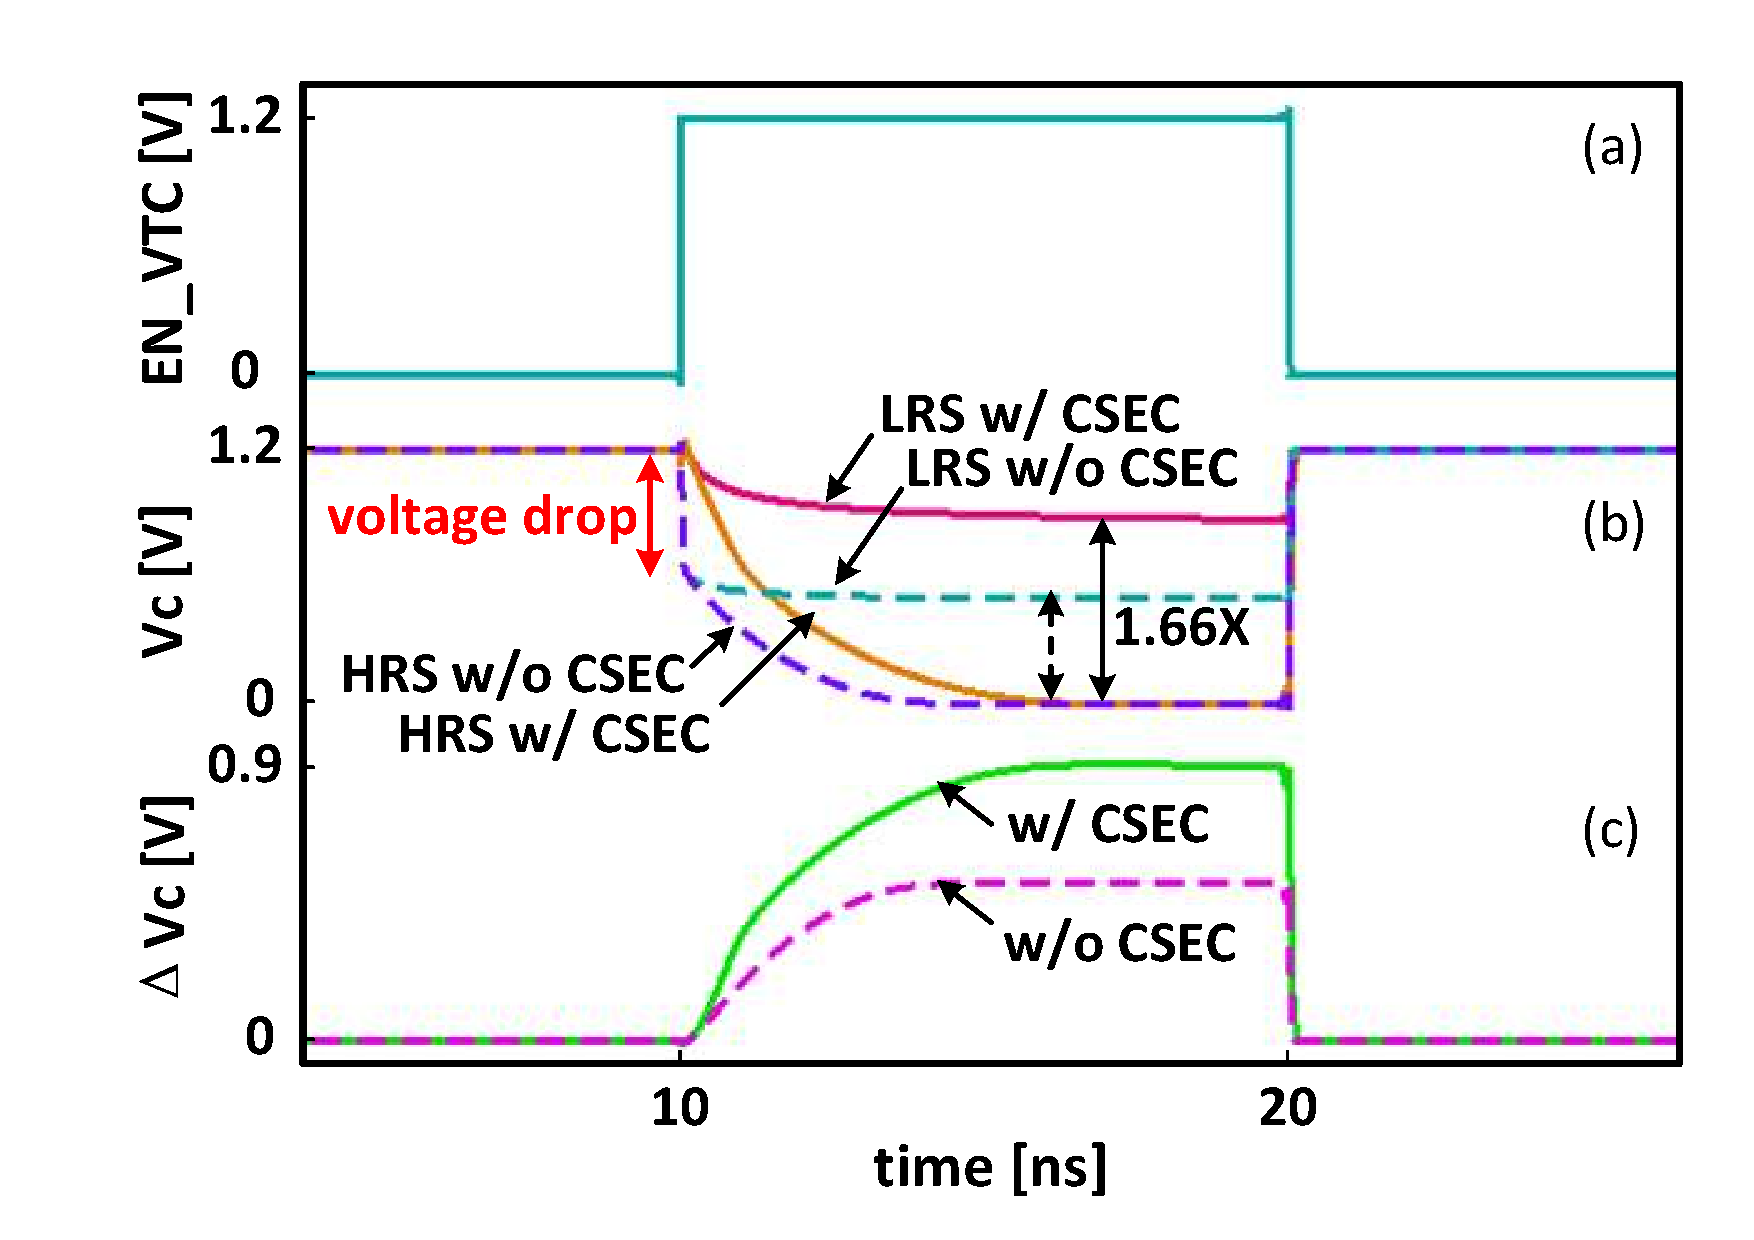
\includegraphics[width=0.48\textwidth]{fig/waveform_CIEF.pdf}}
\caption{
Voltage margin with and without CSEC in a typical case. (a) Voltage to time conversion enable signal $EN\_VTC$; (b) The capacitor node voltage $V_C$ without CSEC (dashed lines) and with CSEC (solid lines); and (c) The voltage difference of $V_C$ when RRAM is in LRS and HRS ($\Delta V_C = V_C(LRS) - V_C(HRS)$). The voltage margin increases 1.66 times with CSEC circuit.
}
\label{fig_CIEF}
\end{figure}

When the enable signal $EN\_VTC$ is inactive, the capacitor node voltage $V_C$ is charged to $V_{DD}$ by the PMOS M$_1$ while the drain voltage of M$_3$ keeps zero because of the pull-down current of M$_3$. At the time of the transition of signal $EN\_VTC$, M$_2$ turns on and draws a high transient current from the node $V_C$ to charge the drain of M$_3$. This leads to a sharp voltage drop of $V_C$ because the pull-up transistor M$_1$ is turned off and the charges stored in the MOS capacitor M$_4$ are shared with the drain capacitor of M$_3$ and the source capacitor of M$_2$. 
The charge sharing-induced voltage drop shrinks the voltage margin for HRS and LRS, and hence risks incorrect sensing and increases the read BER, as the dashed lines are shown in Fig. \ref{fig_CIEF}. 
This charge sharing-induced error is severer when the size of M$_3$ is large considering the large parasitic capacitor at the drain of M$_3$.
% shrinking memory window

Avoiding the charge sharing-induced error benefits robust and accurate sensing by widening the margin of capacitor node voltage $V_C$ in different resistance states (i.e., HRS and LRS).
A charge sharing-induced error compensation (CSEC) scheme is proposed to compensate for the charge and eliminate the voltage drop of $V_C$, as shown in Fig. \ref{fig_prop_circuit}. The two inverters provide a short propagation delay. Driven by the signal that is delayed by $EN\_VTC$, M$_5$ provides an extra charge current at the beginning of the signal $EN\_VTC$ goes high. As a result, the $V_C$ keeps $V_{DD}$ and holds the charge during the transition of $EN\_VTC$. 
It is to be noted that the size of $M_5$ should match the size of $M_4$ to balance the pull-up and pull-down currents for proper charge compensation. If the size of $M_5$ is too small, the voltage drop cannot be compensated completely. On the contrary, an overshoot voltage appears at the rising edge of {EN\_VTC} if the size of $M_5$ is too large.

The comparison of the discharge voltage $V_C$ in different resistance states is shown in Fig. \ref{fig_CIEF}. A 1.66$\times$ voltage margin is achieved with the proposed CSEC circuit. The enlarged sensing window can accommodate wider variations arising from the RRAM devices and other parts of the sensing circuit, improving the read reliability and reducing the read BER.   
Avoiding the charge sharing-induced error is beneficial not only to voltage margin improvement but also to energy saving for the subsequent shaping inverter. That is because $V_C$ in LRS (see Fig. \ref{fig_CIEF}) is much closer to the trip voltage of the following inverter if without CSEC, consuming a large short-circuit current during the sensing period.

\begin{figure}[!t]
\centerline
{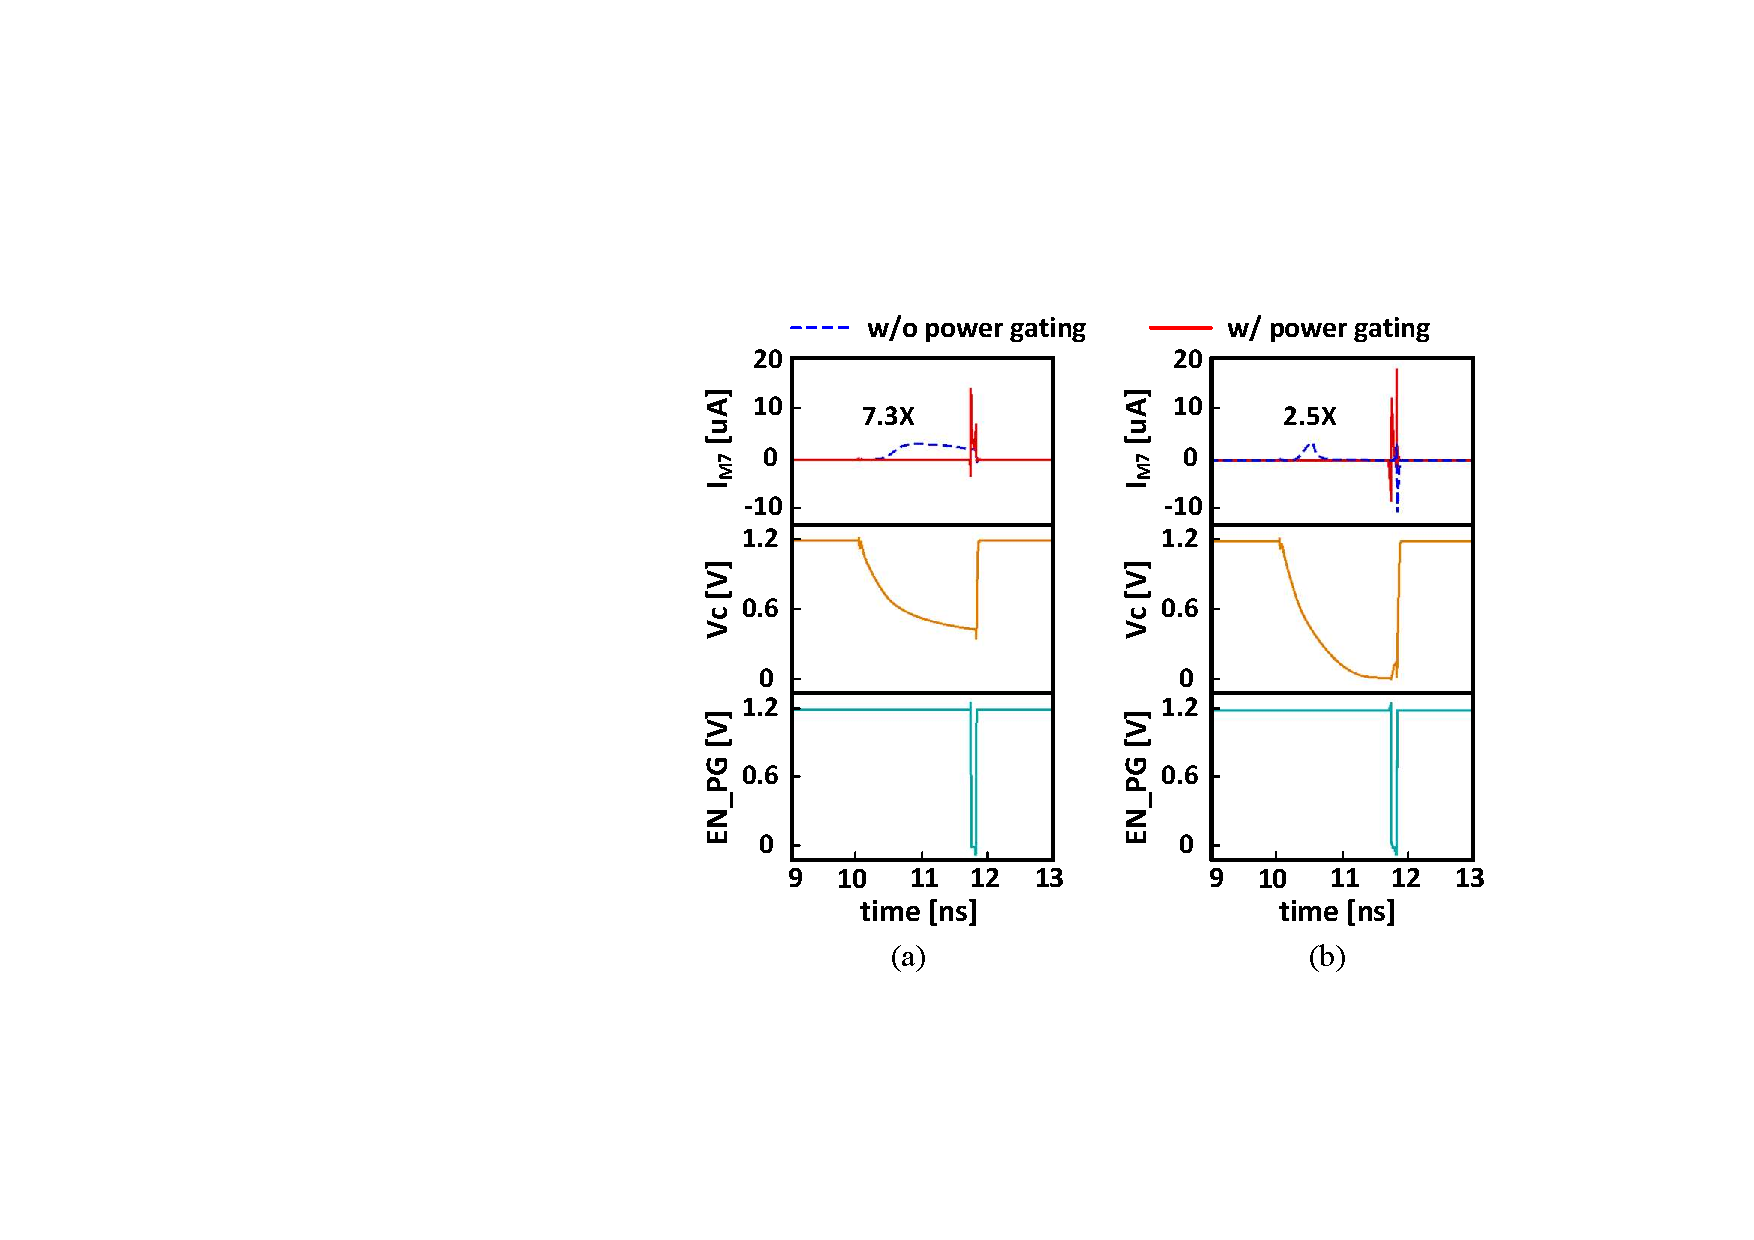
\includegraphics[width=0.5\textwidth]{fig/power_gating_current.pdf}}
\caption{Comparison of the current consumption of the shaping inverter with and without power gating. (a) $V_C$ is around $V_{DD}/2$. (b) $V_C$ is close to zero.}
\label{fig_powergating}
\end{figure}


\subsection{Power Gating Technique}
The inverter (M$_7$ and M$_8$) after VTC behaves as a voltage detector and signal shaper. The trip voltage $V_{TRIP}$ of this inverter is compared with the output of the VTC. As a result, the slow-edged capacitor node voltage $V_C$ is shaped by the cascaded inverters to generate a sharp-edged signal $V_{out}$ at the input of the subsequent DFF.

The energy drawn by the shaping inverter $E_{shaping}$ is dominated by its short-circuit current associated with the slow transition of the discharge voltage $V_C$, as determined by the operation of M$_3$ in the sub-threshold region (see Fig. \ref{fig_prop_circuit}(a)).
By inserting a PMOS sleep transistor M$_6$, the power gating inverter (PGI) is enabled only when the gate signal of M$_6$ is activated.
The gate signal $EN\_PG$ is generated directly by the combination logic from  the timing control loop. $EN\_PG$ is low active for the PGI and its positive edge triggers the DFF (see Fig. \ref{fig_prop_circuit}).
The value of $V_C$ depends on the discharge current $I_{DISCH}$ (determined by the size of $M_3$ for the same $V_{BL}$) and the discharge time $T_{DISCH}$. A short period of short-circuit current is consumed only when $EN\_PG$ is enabled and $V_C$ is close to the trip voltage of the shaping inverter (i.e., around $V_{DD}/2$). It can achieve short-circuit-current-free if $EN\_PG$ is enabled when $V_C$ is much less than the threshold voltage of M$_8$ (i.e., close to zero). 
% but with the penalty of longer sensing time. 

Fig. \ref{fig_powergating} illustrates the transition of the discharge voltage $V_C$ and the current consumption with and without power gating. 
We can see the power gating achieves $7.3\times$ and $2.5\times$ energy saving for the case of $V_C$ around $V_{DD}/2$ and zero, respectively. 
% $V_C$ is modulated by size of $M_3$.
To shape the voltage $V_C$ into a sharp edge signal at the input of the DFF, \cite{trinh2018time} adopted a $4\times$ minimum-sized inverter, resulting in a large shaping current ($\approx 50~\rm \micro A$ averaging). In this work, two cascaded inverters are used to shape the voltage and make the sensing margin positive (i.e., LRS of RRAM results in output high). By this, minimum-sized transistors are used in the PGI with the average current less than $5~\rm \micro A$ during sensing. 
The transient current spikes are caused by gate tunneling leakage when the gate voltage goes high, which is negligible compared to the shaping power. 
% Avoiding the short-circuit current is beneficial to not only power consumption but also phase linearity.

\subsection{Dual-mode Timing Controller}

% \begin{figure}[!t]
% \centerline
% {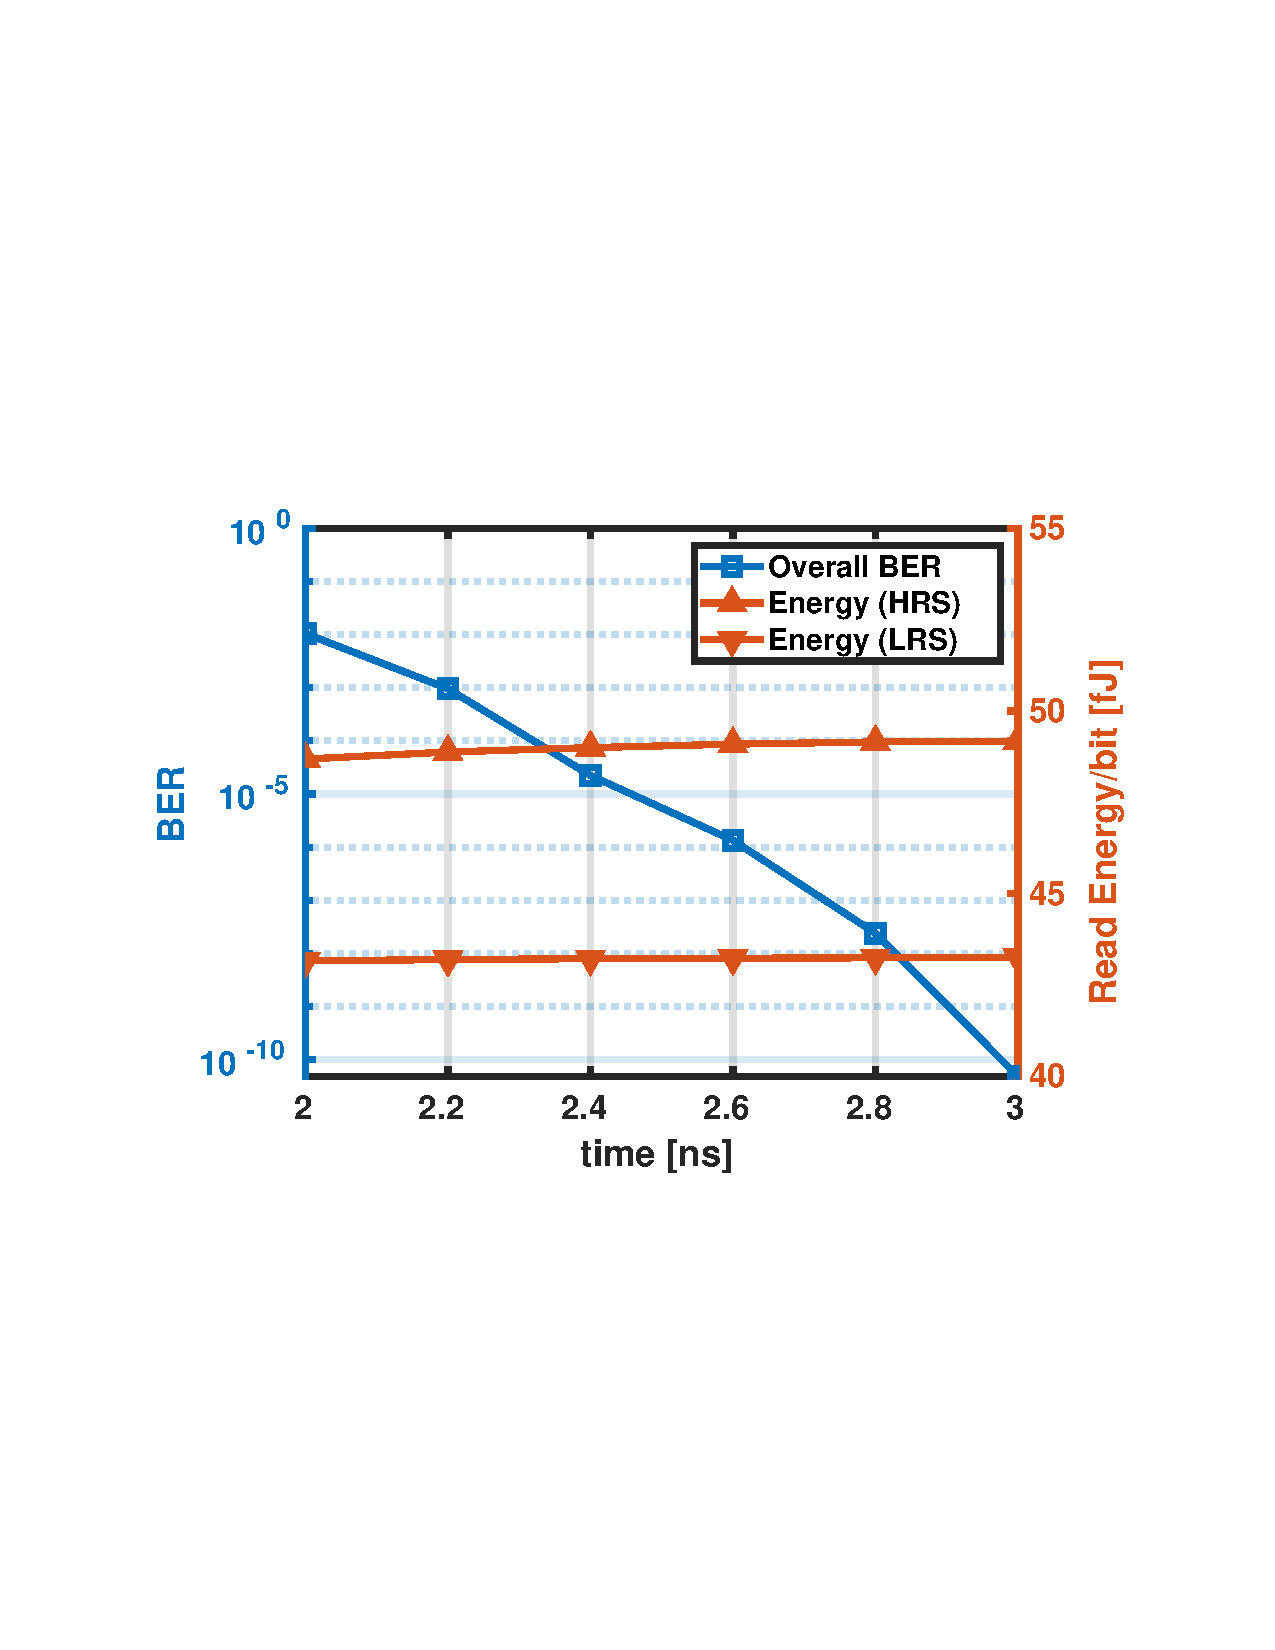
\includegraphics[width=0.45\textwidth]{fig/ber_delay_energy.pdf}}
% \caption{BER and read energy per bit of the proposed time-based sensing with respect to the delay time $T_1$.}
% \label{fig_ber_delay}
% \end{figure}

\begin{figure}[!t]
    \centering
    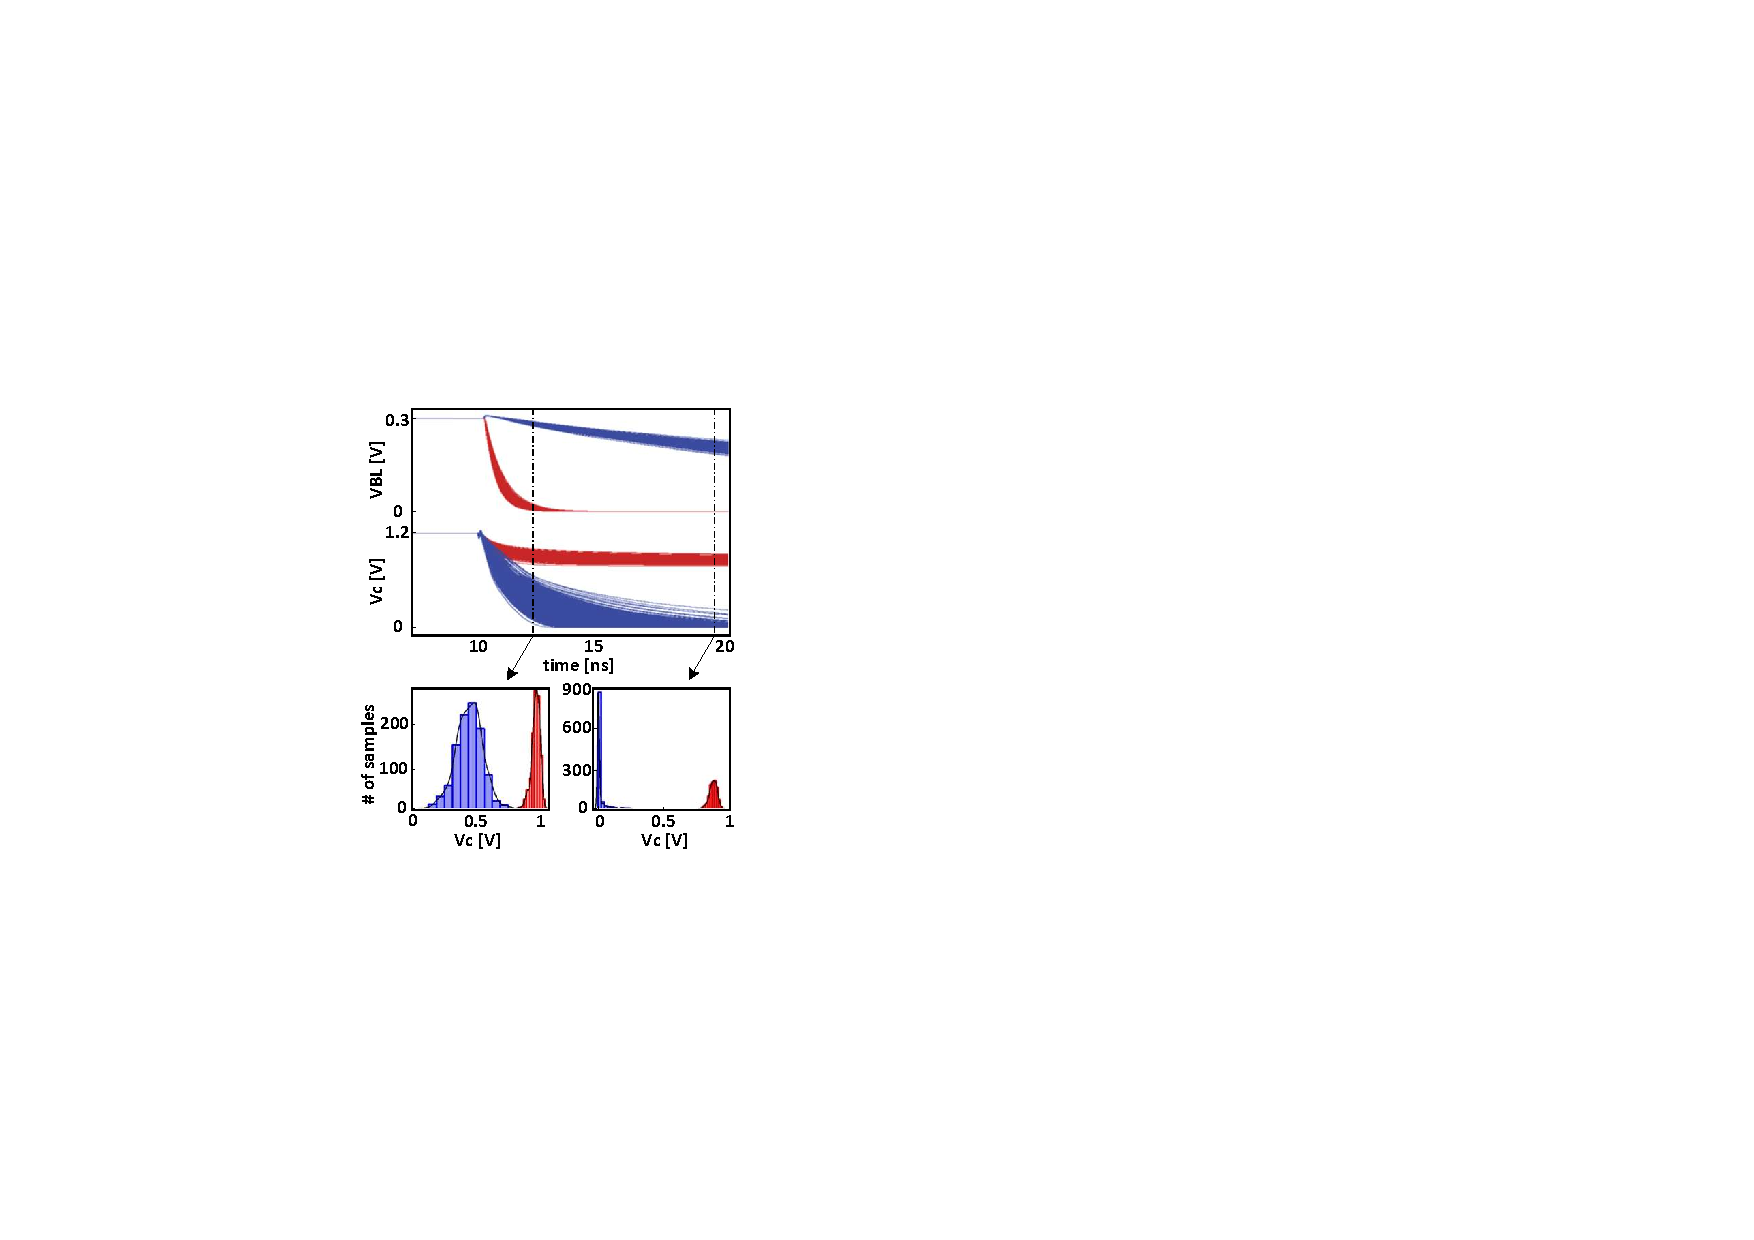
\includegraphics[width=0.4\textwidth]{fig/VC_MC_new.pdf}
    \caption{Monte Carlo simulation of $V_{BL}$ and $V_C$ in different RRAM states generated from 1000 runs. Transient waveforms (top panel) and histogram of $V_C$ at two different times (bottom panel).}
    \label{fig_vc}
\end{figure}
     
\begin{figure}[!t]
    \centering
    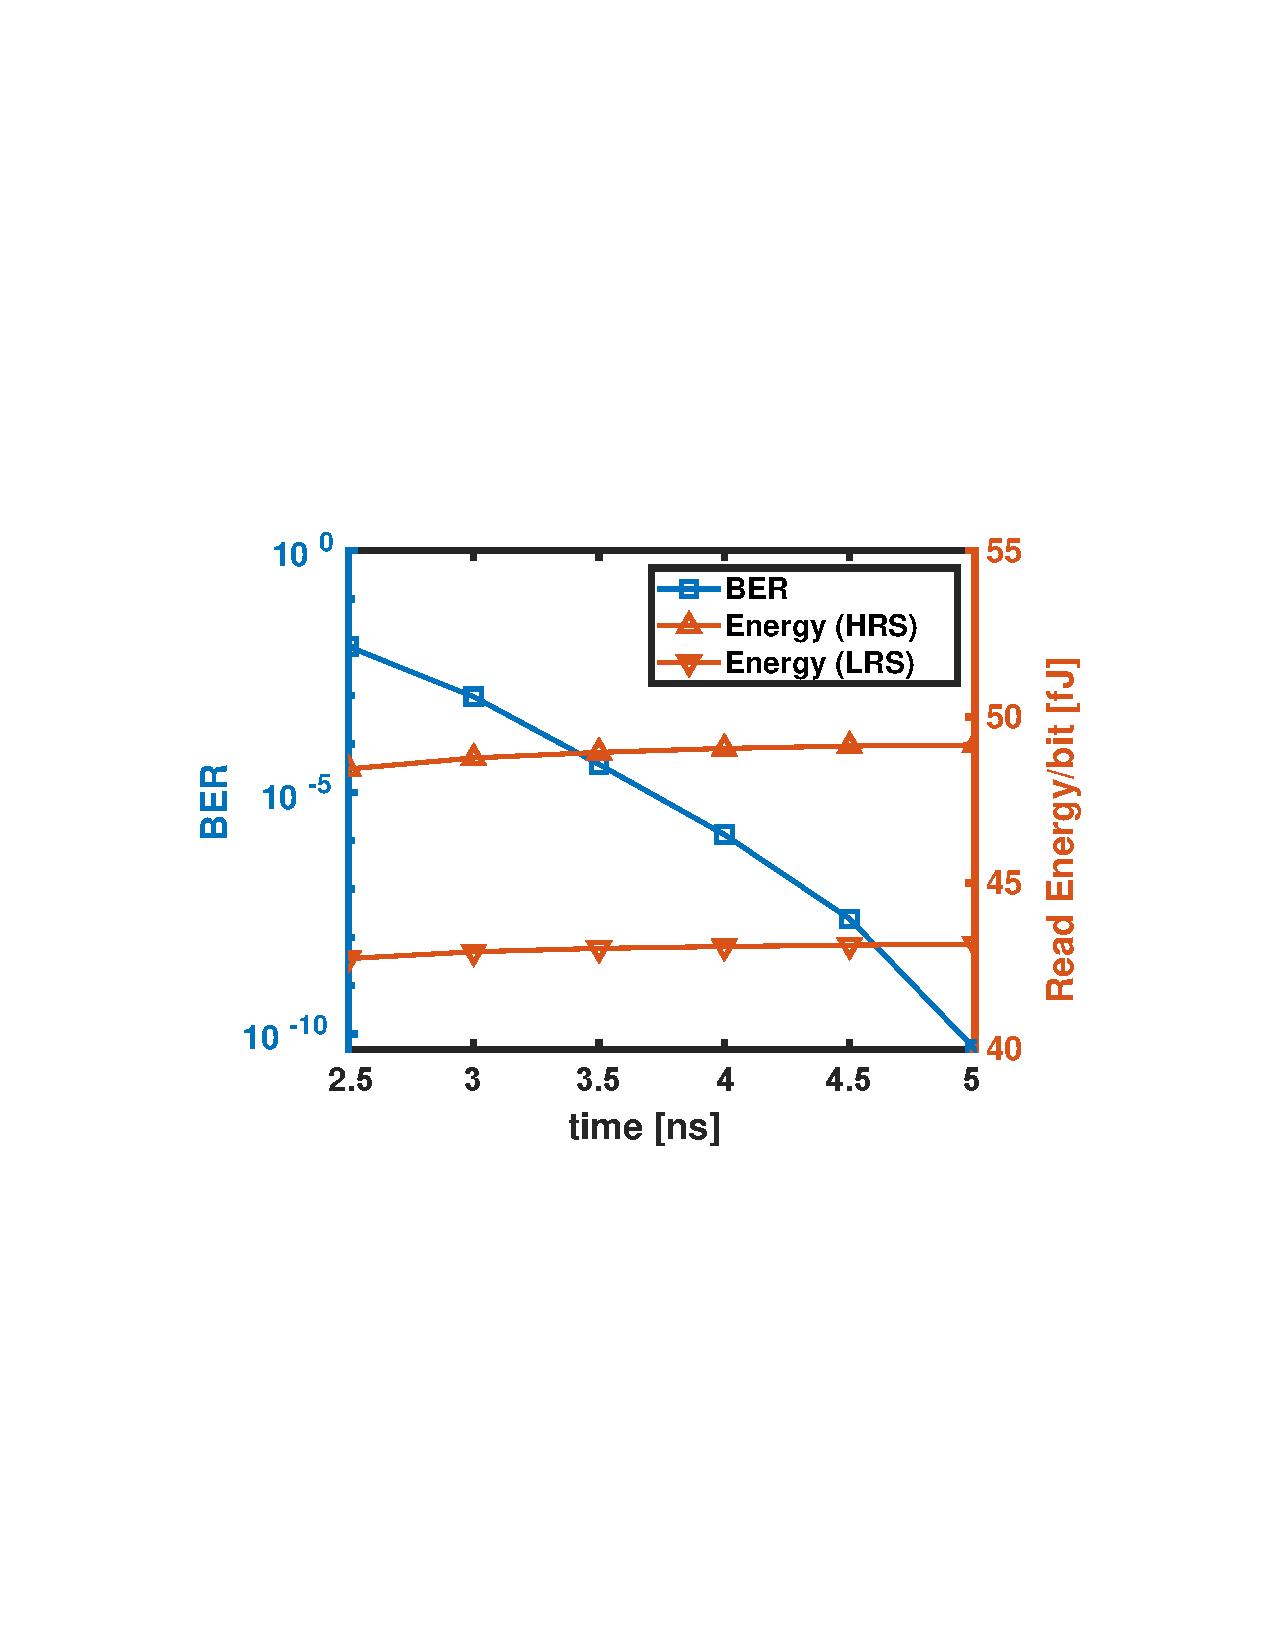
\includegraphics[width=0.45\textwidth]{fig/ber_delay_energy_new.pdf}
    \caption{
    BER and read energy per bit of the proposed time-based sensing with respect to the delay time $T_1$.}
    \label{fig_ber_delay}
\end{figure}


%% figure in the next section
\begin{figure*}[!t]
\centerline
{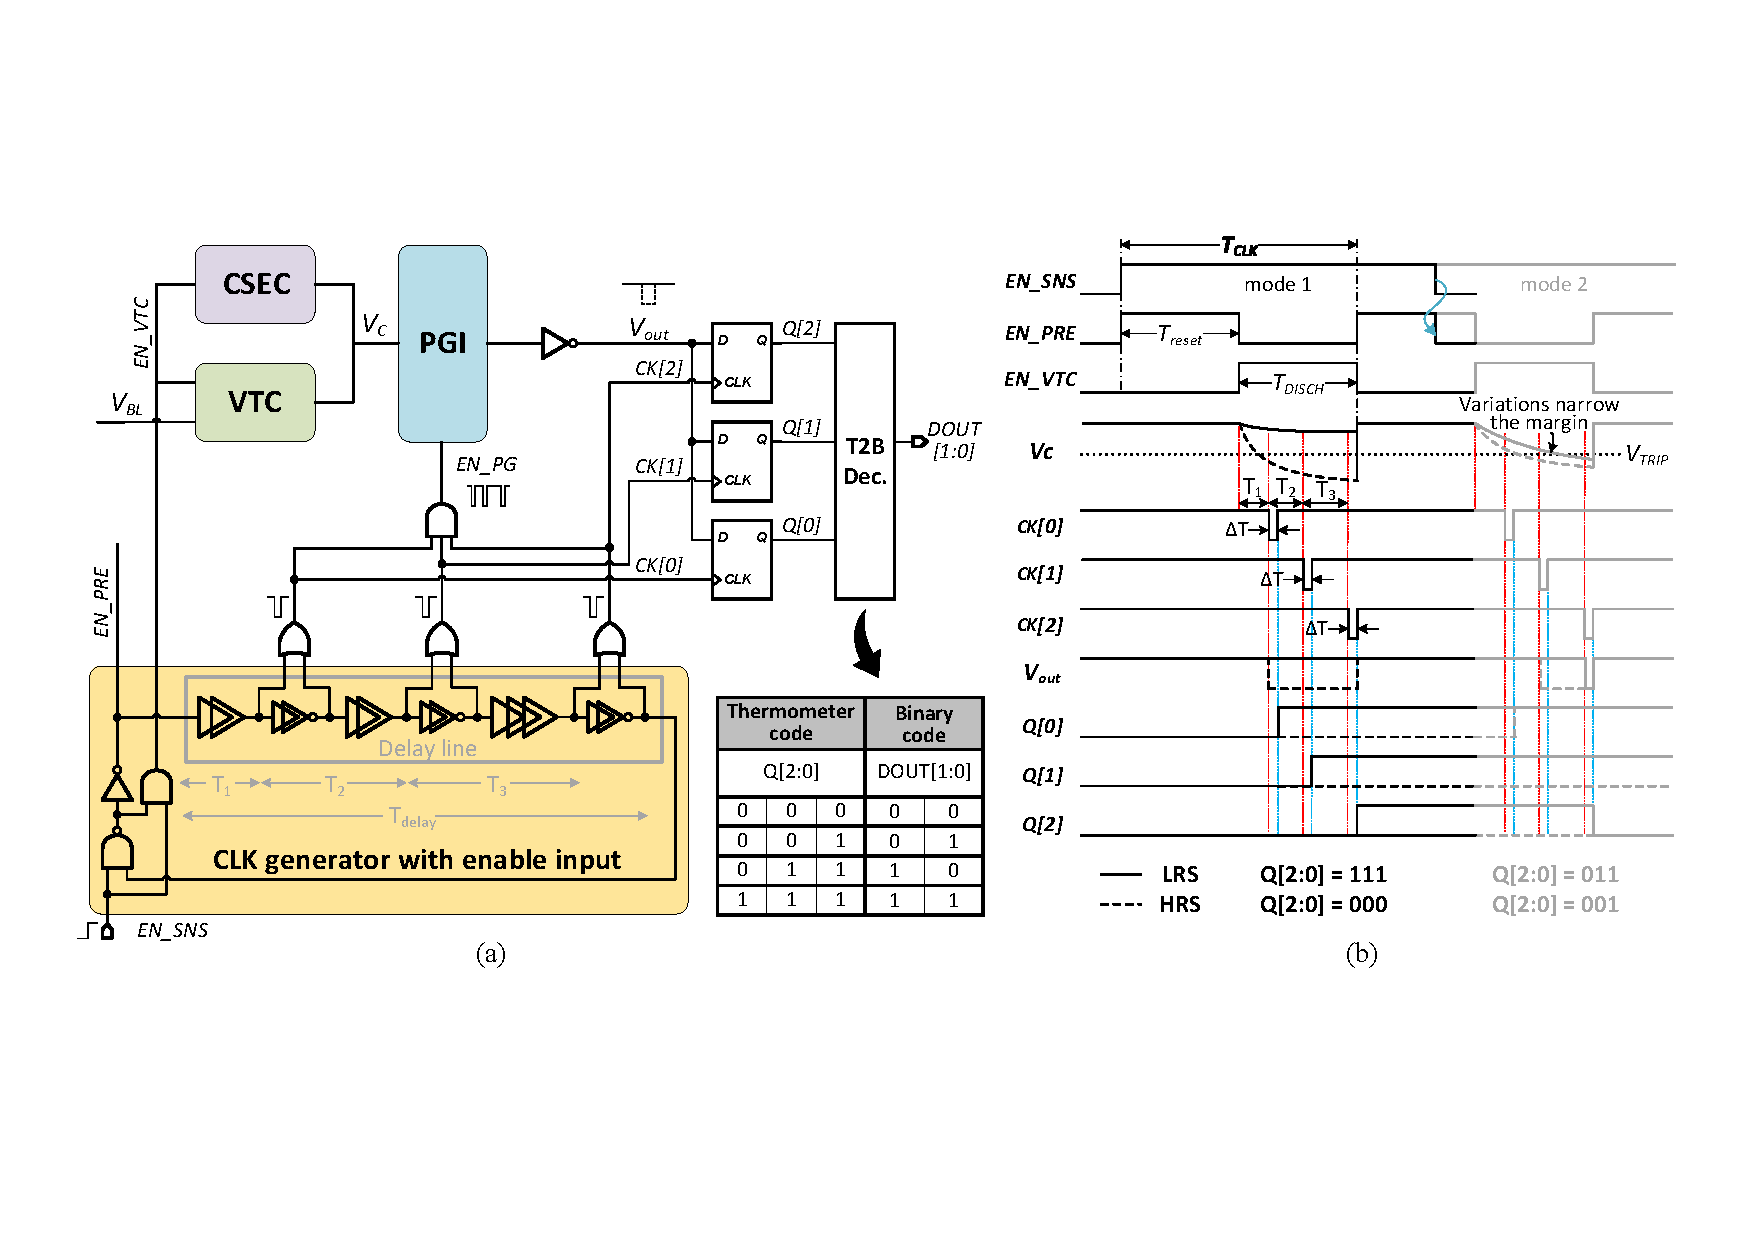
\includegraphics[width=0.98\textwidth]{fig/time_sensing_multiple_new.pdf}}
\caption{Extension of the proposed time-based sensing to multi-level sensing: (a) circuit diagram and the truth table of thermometer code to binary code (T2B) decoder. (b) Typical waveforms of critical nodes for different RRAM states (LRS and HRS) in different readout modes.}
\label{fig_multiple_sensing}
\end{figure*}

The dual-mode timing control block consists of a delay line and a combination logic to generate the control signals for the proposed time-based sense amplifier (TSA). The output of the delay line is fed back to its input as a closed-loop to derive a ring oscillator for automatic reading. The clock generator loop is controlled by the enable signal $EN\_SNS$.

The clock period of the oscillator $T_{CLK}$ depends on the total delay time of the loop. For a stable ring oscillator, the signal must go through each of the delay stages twice to provide one period of oscillation \cite{zhang2021cco}, which can be evaluated by
\begin{align}
\label{eq_clk}
T_{CLK} \approx 2(T_1+\Delta T)
\end{align}
where $T_1$ denotes the delay time of the delay line for RRAM state sensing and voltage developing, and $\Delta T$ denotes the short enable time for PGI to shape the voltage and for the DFF to latch the data, as depicted in Fig. \ref{fig_prop_circuit}(b). 
Although smaller $\Delta T$ consumes lower energy in the PGI, $\Delta T$ should be larger than the propagation delay of the shaping inverters from $V_C$ to $V_{out}$ in order to sample correctly for the DFF.

Fig. \ref{fig_vc} shows 1000 runs MC simulation results of transient $V_{BL}$ and $V_C$ for RRAM in different states, as well as the histogram distribution of $V_C$ at a shorter and longer delay time.
Interestingly, $V_C$ in LRS keeps constant after a short time of discharge because $V_{BL}$ is quickly pulled down to the ground by the low resistance of RRAM. Therefore, the voltage difference of $V_C$ in LRS and HRS increases with the discharge time. 
The discharge time $T_1$ determines the read BER and the read energy, as shown in Fig. \ref{fig_ber_delay}. With a longer delay time, $V_C$ corresponding to HRS goes as low as zero and the voltage window of different states enlarges gradually. As a result, the read operation becomes more reliable and the BER decreases. On the other hand, the sensing energy is almost constant for both HRS and LRS (lower than 50 fJ) over the delay time due to the power gating employed. It is noteworthy that the read energy in HRS consumes $\sim 6$ fJ higher than the read energy in LRS. The extra energy is consumed for resetting $V_C$, considering $V_C$ is discharged much lower in HRS (see Fig. \ref{fig_vc}).
Only negligible static power is consumed during the extended delay time.
% It is important to note, however, extending the delay time too much will increase $BER_{LRS}$, and hence degrade the overall BER.
Theoretically, extending the delay time too much will increase $BER_{LRS}$, and hence degrade the overall BER, as shown in Fig. \ref{fig_BER_probability}. 
In our design, the size of the MOS transistor in the 1T1R bitcell is $W/L$ = 360 nm/40 nm, leading to the maximum discharge current of 100 (85) $\rm \micro$A for bitcell in LRS under a precharge voltage of 400 (300) mV. $V_{BL}$ would be discharged to 100 mV within 2.5 ns, resulting in $V_C$ kept high in LRS and eliminating the limitation of $BER_{LRS}$ in practice. It is important to note that the read access time increases with lower precharge voltage since it takes a longer discharge time to discriminate $V_C$.

The dual-mode timing control logic supports two different readout operation modes according to the pulse width of the enable signal $EN\_SNS$, as listed at the bottom of Fig. \ref{fig_prop_circuit}(a).
\begin{enumerate}
\item[1)] Single Readout Mode\\
When the pulse width of $EN\_SNS$ is set $T_{CLK}<T_{EN\_SNS}<\frac{3}{2}T_{CLK}$, the VTC enable signal $EN\_VTC$ is enabled only once and therefore, the TSA read the state one time, as the black waveforms shown in Fig. \ref{fig_prop_circuit}(b). When $EN\_SNS$ goes low, the TSA is reset for the next sensing.
\item[2)] Multiple Readout Mode\\
If $T_{EN\_SNS} \geq 2T_{CLK}$, the timing control loop activates $EN\_PRE$ and $EN\_VTC$ alternately and the TSA reads the state consecutively, as the grey waveforms shown in Fig. \ref{fig_prop_circuit}(b). With no external controller required, it can read the whole memory array automatically by using the $T_{CLK}$ as the system read clock. Besides, this is also useful in the case of successively reading the same bitcell multiple times for statistical analysis.  
\end{enumerate}



The dual-mode timing controller block includes many buffers in the delay line and correspondingly consumes significant energy (39\%) and areas (43\%). In this work, a $512 \times 512$ 1T1R array is designed, and the timing controller block is shared with all TSAs. Therefore, the overhead distributed into each TSA becomes negligible. 
